
\documentclass[11pt, oneside]{book}

%%%%%%%%%%%%%%Include Packages%%%%%%%%%%%%%%%%%%%%%%%%%%
\usepackage{xcolor}
\usepackage{mathtools}
\usepackage[a4paper, total={6in, 8in}, margin=1.25in]{geometry}
\usepackage{amsmath}
\usepackage{amssymb}
\usepackage{paralist}
\usepackage{rsfso}
\usepackage{amsthm}
\usepackage{wasysym}
\usepackage[inline]{enumitem}   
\usepackage{hyperref}
\usepackage{tocloft}
\usepackage{wrapfig}
\usepackage{titlesec}
\usepackage{colortbl}
\usepackage{stackengine} 
\usepackage{listings}
%%%%%%%%%%%%%%%%%%%%%%%%%%%%%%%%%%%%%%%%%%%%%%%%%%%%%%%%



%%%%%%%%%%%%%%%Code%%%%%%%%%%%%%%%%%%%%%%%%%%%%%%%%%%%%%
\definecolor{codegreen}{rgb}{0,0.6,0}
\definecolor{codegray}{rgb}{0.5,0.5,0.5}
\definecolor{codepurple}{rgb}{0.58,0,0.82}
\definecolor{backcolour}{rgb}{0.95,0.95,0.92}

\lstdefinestyle{mystyle}{
    backgroundcolor=\color{backcolour},   
    commentstyle=\color{codegreen},
    keywordstyle=\color{magenta},
    numberstyle=\tiny\color{codegray},
    stringstyle=\color{codepurple},
    basicstyle=\ttfamily\footnotesize,
    breakatwhitespace=false,         
    breaklines=true,                 
    captionpos=b,                    
    keepspaces=true,                 
    numbers=left,                    
    numbersep=5pt,                  
    showspaces=false,                
    showstringspaces=false,
    showtabs=false,                  
    tabsize=2
}
%%%%%%%%%%%%%%%%%%%%%%%%%%%%%%%%%%%%%%%%%%%%%%%%%%%%%%%%

%%%%%%%%%%%%%%%Chapter Setting%%%%%%%%%%%%%%%%%%%%%%%%%%
\definecolor{gray75}{gray}{0.75}
\newcommand{\hsp}{\hspace{20pt}}
\titleformat{\chapter}[hang]{\Huge\bfseries}{\thechapter\hsp\textcolor{gray75}{$\mid$}\hsp}{0pt}{\Huge\bfseries}
%%%%%%%%%%%%%%%%%%%%%%%%%%%%%%%%%%%%%%%%%%%%%%%%%%%%%%%%

%%%%%%%%%%%%%%%%%Theorem environments%%%%%%%%%%%%%%%%%%%
\newtheoremstyle{break}
  {\topsep}{\topsep}%
  {\itshape}{}%
  {\bfseries}{}%
  {\newline}{}%
\theoremstyle{break}
\theoremstyle{break}
\newtheorem{axiom}{Axiom}
\newtheorem{thm}{Theorem}[section]
\renewcommand{\thethm}{\arabic{section}.\arabic{thm}}
\newtheorem{lem}{Lemma}[thm]
\newtheorem{cor}{Corollary}[thm]
\newtheorem{defn}{Definition}[thm]
\newenvironment{indEnv}[1][Proof]
  {\proof[#1]\leftskip=1cm\rightskip=1cm}
  {\endproof}
%%%%%%%%%%%%%%%%%%%%%%%%%%%%%%%%%%%%%%%%%%%%%%%%%%%%%%


%%%%%%%%%%%%%%%%%%%%%%%Integral%%%%%%%%%%%%%%%%%%%%%%%
\def\upint{\mathchoice%
    {\mkern13mu\overline{\vphantom{\intop}\mkern7mu}\mkern-20mu}%
    {\mkern7mu\overline{\vphantom{\intop}\mkern7mu}\mkern-14mu}%
    {\mkern7mu\overline{\vphantom{\intop}\mkern7mu}\mkern-14mu}%
    {\mkern7mu\overline{\vphantom{\intop}\mkern7mu}\mkern-14mu}%
  \int}
\def\lowint{\mkern3mu\underline{\vphantom{\intop}\mkern7mu}\mkern-10mu\int}
%%%%%%%%%%%%%%%%%%%%%%%%%%%%%%%%%%%%%%%%%%%%%%%%%%%%%%



\newcommand{\R}{\mathbb{R}}
\newcommand{\N}{\mathbb{N}}
\newcommand{\Z}{\mathbb{Z}}
\newcommand{\Q}{\mathbb{Q}}
\newcommand{\C}{\mathbb{C}}
\newcommand{\T}{\mathcal{T}}
\newcommand{\M}{\mathcal{M}}
\newcommand{\Symm}{\text{Symm}}
\newcommand{\Alt}{\text{Alt}}
\newcommand{\Int}{\text{Int}}
\newcommand{\Bd}{\text{Bd}}
\newcommand{\Power}{\mathcal{P}}
\newcommand{\ee}[1]{\cdot 10^{#1}}
\newcommand{\spa}{\text{span}}
\newcommand{\sgn}{\text{sgn}}
\newcommand{\degr}{\text{deg}}
\newcommand{\pd}{\partial}
\newcommand{\that}[1]{\widetilde{#1}}
\newcommand{\lr}[1]{\left(#1\right)}
\newcommand{\vmat}[1]{\begin{vmatrix} #1 \end{vmatrix}}
\newcommand{\bmat}[1]{\begin{bmatrix} #1 \end{bmatrix}}
\newcommand{\pmat}[1]{\begin{pmatrix} #1 \end{pmatrix}}
\newcommand{\rref}{\xrightarrow{\text{row\ reduce}}}
\newcommand{\txtarrow}[1]{\xrightarrow{\text{#1}}}
\newcommand\oast{\stackMath\mathbin{\stackinset{c}{0ex}{c}{0ex}{\ast}{\Circle}}}
\newcommand{\txt}{Wald's \textit{General Relativity}}

\newcommand{\note}{\color{red}Note: \color{black}}
\newcommand{\remark}{\color{blue}Remark: \color{black}}
\newcommand{\example}{\color{green}Example: \color{black}}
\newcommand{\exercise}{\color{green}Exercise: \color{black}}

%%%%%%%%%%%%%%%%%%%%%%Roman Number%%%%%%%%%%%%%%%%%%%%%%%
\makeatletter
\newcommand*{\rom}[1]{\expandafter\@slowromancap\romannumeral #1@}
\makeatother
%%%%%%%%%%%%%%%%%%%%%%%%%%%%%%%%%%%%%%%%%%%%%%%%%%%%%%%%%

%%%%%%%%%%%%%table of contents%%%%%%%%%%%%%%%%%%%%%%%%%%%%
%\setlength{\cftchapindent}{0em}
%\cftsetindents{section}{2em}{3em}
%
%\renewcommand\cfttoctitlefont{\hfill\huge\bfseries}
%\renewcommand\cftaftertoctitle{\hfill\mbox{}}
%
%\setcounter{tocdepth}{2}
%%%%%%%%%%%%%%%%%%%%%%%%%%%%%%%%%%%%%%%%%%%%%%%%%%%%%%%%%%


%%%%%%%%%%%%%%%%%%%%%Footnotes%%%%%%%%%%%%%%%%%%%%%%%%%%%
\newcommand\blfootnote[1]{%
  \begingroup
  \renewcommand\thefootnote{}\footnote{#1}%
  \addtocounter{footnote}{-1}%
  \endgroup
}
%%%%%%%%%%%%%%%%%%%%%%%%%%%%%%%%%%%%%%%%%%%%%%%%%%%%%%%%%

%%%%%%%%%%%%%%%%%%%%%Section%%%%%%%%%%%%%%%%%%%%%%%%%%%%%
\makeatletter
\def\@seccntformat#1{%
  \expandafter\ifx\csname c@#1\endcsname\c@section\else
  \csname the#1\endcsname\quad
  \fi}
\makeatother
%%%%%%%%%%%%%%%%%%%%%%%%%%%%%%%%%%%%%%%%%%%%%%%%%%%%%%%%%

%%%%%%%%%%%%%%%%%%%%%%%%%%%%%%%%%%%Enumerate%%%%%%%%%%%%%%
\makeatletter
% This command ignores the optional argument 
% for itemize and enumerate lists
\newcommand{\inlineitem}[1][]{%
\ifnum\enit@type=\tw@
    {\descriptionlabel{#1}}
  \hspace{\labelsep}%
\else
  \ifnum\enit@type=\z@
       \refstepcounter{\@listctr}\fi
    \quad\@itemlabel\hspace{\labelsep}%
\fi}
\makeatother
\parindent=0pt
%%%%%%%%%%%%%%%%%%%%%%%%%%%%%%%%%%%%%%%%%%%%%%%%%%%%%%%%%%



\begin{document}

	\begin{titlepage}
		\begin{center}
			\vspace*{0.5cm}
			\Huge \color{red}
				\textbf{Homework 7}\\
			\vspace{0.5cm}			
			\Large \color{black}
			Physics 542 - Quantum Optics\\
			Professor Alex Kuzmich
			\vspace{1.5cm}

			
\includegraphics[scale=1.15]{hmm.pdf}
			
			
			\vspace{2cm}
			\LARGE
				\textbf{Jinyan Miao}\\
				\hfill\break
				\LARGE Fall 2023\\
			\vspace{1cm}

		\vspace*{\fill}
		\end{center}			
	\end{titlepage}

\chapter{}
First we consider the case of $N=2$ and $S = 1$, in which case we have (from Eq.\,(11a) on C. Genes and P. Berman, \textit{Spin squeezing via atom-cavity field coupling}, Phys. Rev. A \textbf{68}, 043809 (2003),)
\begin{align}
\langle \hat{S}_x^2\rangle = \frac{1}{2} + \sum_{n=0}^\infty \left( \frac{1}{2}|c_{0,n}|^2 + c_{1,n}c_{-1,n}\right)\,,
\end{align}
where $c_{m,n}$ is the coefficient in the interaction representation of the state
\begin{align}
|\psi(t)\rangle = \sum_{m=-N/2}^{N/2} \sum_{n=0}^\infty c_{m,k}e^{-i\omega (m+n)t}|m,n\rangle\,,
\end{align}
and here $m$ labels the value of $S_z$ and $n$ labels the number of photons in the cavity field.  Spin squeezing happens when we have
\begin{align}
\xi_{x} = \frac{\sqrt{N \langle \hat{S}^2_x\rangle}}{|\langle \mathbf{S}\rangle |}<1\,,
\end{align}
thus in this case we would like to have $\langle S_x^2\rangle$ for spin squeezing, which is possible only when we have some $c_{1,n}c_{-1,n} < 0$ as $|c_{0,n}|$ is non-negative. From Eq.\,(21.57) from Berman's text \textit{Principles of Laser Spectroscopy and Quantum Optics}, we know that
\begin{align}
c_{1,n}c_{-1,n}\propto c_{k}c_{k+2}
\end{align}
where $c_k$ are the initial state amplitudes for the field. Thus it is required to have $c_{k}c_{k+2} \neq 0$ in order for spin squeezing happening, thus requiring coherence between states differing by two. To generalize this effect to general $N$ atoms system, it suffices to examine the form of $\hat{S}_x^2$ and the interaction Hamiltonian between the atoms and the field. The interaction Hamiltonian of the system is given by
\begin{align}
\hat{H}_{\text{int}} = \hbar g\left( \hat{S}_+ \hat{a} + \hat{S}_-\hat{a}^\dagger\right)\,,
\end{align}
thus it is well-expected that the evolution of the wavefunction of the system, Eq.\,(1.2), satisfies $c_{m-1,k}\propto c_k$ and $c_{m+1,k}\propto c_{k+2}$, and thus Eq.\,(1.4) is again satisfied. Now from the form of $\hat{S}_{x}^2$, Eq.\,(21.41) from Berman's text \textit{Principles of Laser Spectroscopy and Quantum Optics},
\begin{align*}
\hat{S}_x^2 = \sum_{i,j=1}^N s_x^is_x^j = \frac{N}{4}+ \sum_{i,j\neq i}^N s_x^i s_x^j\,,
\end{align*}
it is expected that the only possible non-positive terms in $\langle S_x^2\rangle$ are of the form $c_{m+1,n}c_{m-1,n}$. Following the argument as in the $N=2$ case proves the result. 

\chapter{}
Here we will show that $[\hat{S}_x, \hat{S}_y] = i \hat{S}_z$, and $\hat{S}_z \hat{S}_+ \neq \hat{S}_+/2$. \\
For cleanness we drop the operator hat in the notations. 
\begin{align*}
S_xS_y = \sum_{j=1}^N s_x^j \sum_{i=1}^N s_y^i = \sum_{i,j = 1}^N s_x^j s_y^i\,,\qquad 
S_y S_x = \sum_{i,j=1}^N s_y^j s_x^i\,.
\end{align*}
Here we have that 
\begin{align*}
s_x s_y &= -\frac{i}{4}\left( s_+ + s_-\right)(s_+ - s_-)  \\
&= -\frac{i}{4}(s_+s_+ - s_+s_- + s_-s_+ - s_-s_-)\\
&= -\frac{i}{4}(|2\rangle\langle 1|2\rangle\langle 1| - |2\rangle\langle 1| 1\rangle\langle 2| + |1\rangle\langle 2|2\rangle\langle 1| - |1\rangle\langle 2|1\rangle\langle 2| )\\
&= \frac{i}{4}\left( |2\rangle\langle 2| - |1\rangle\langle 1|\right)\,.
\end{align*}
\begin{align*}
s_y s_x &= -\frac{i}{4}(s_+ - s_-) \left( s_+ + s_-\right) \\
&= -\frac{i}{4}\left(s_+s_+ + s_+s_- - s_-s_+ -s_-s_- \right)\\
&= \frac{i}{4}\left( s_-s_+ - s_+s_-\right) \\
&= \frac{i}{4}\left(|1\rangle\langle 1| - |2\rangle\langle 2| \right)\,.
\end{align*}
Thus we conclude
\begin{align*}
[s_y,s_y] = \frac{i}{2}\left( |2\rangle\langle 2| - |1\rangle\langle 1|\right) = i s_z\,.
\end{align*}
As single-spin operators only operate on that single spin, thus $[s_x^j,s_y^i] = 0$ for $i \neq j$.  It follows that we have
\begin{align*}
[S_x,S_y] =S_x S_y - S_yS_x = \sum_{i,j=1}^N s_x^js_y^i- s_y^js_x^i = \sum_{i=1}^N s_x^is_y^i- s_y^is_x^i = \sum_{i=1}^N [s_x^i,s_y^i] = \sum_{i=1}^N is_z = iS_z
\end{align*}
Now we see here
\begin{align*}
s_zs_+ = \frac{1}{2}\left( |2\rangle\langle 2| - |1\rangle\langle 1| \right) | 2\rangle\langle 1| = \frac{1}{2}\left( |2\rangle\langle 1| \right) = \frac{1}{2}s_+\,.
\end{align*}
While on the other hand
\begin{align*}
\frac{1}{2} S_+ =\frac{1}{2} \sum_{i=1}^N s_+^i\,,
\end{align*}
but
\begin{align*}
S_zS_+ = \sum_{i=1}^N s_z^i \sum_{j=1}^N s_+^j = \sum_{i,j=1}^N s_z^is_+^j &= \sum_{i=1}^N s_z^i s_+^i + \sum_{i\neq j}^N s_z^is_+^j  \\
&=\left(\frac{1}{2} \sum_{i=1}^N s_+ \right)+ \sum_{i\neq j}^N s_z^is_+^j = \frac{1}{2}S_+ + \sum_{i\neq j}^N s_z^is_+^j \neq \frac{1}{2}S_+
\end{align*}
as the term $\sum_{i\neq j}^N s_z^is_+^j$ does not vanish. 



\chapter{}
Here Eq.\,(21.45) from Berman's text \textit{Principles of Laser Spectroscopy and Quantum Optics} reads
\begin{align*}
\xi_x = \frac{\sqrt{N}\sqrt{\langle S_x^2\rangle}}{|\langle \mathbf{S}\rangle|}
\end{align*}
Again, from Eq.\,(11a) on C. Genes and P. Berman, \textit{Spin squeezing via atom-cavity field coupling}, Phys. Rev. A \textbf{68}, 043809 (2003), we have that 
\begin{align*}
(\Delta S_x)^2 = \frac{1}{2}+ \sum_{n=0}^\infty \left( \frac{1}{2}|c_{0,n}|^2 + c_{1,n}c_{-1,n}\right)\,,
\end{align*}
with Eq.\,(21.57) from Berman's text \textit{Principles of Laser Spectroscopy and Quantum Optics}, we compute $(\Delta S_x)^2$ up to the order of $\alpha^2$,
\begin{align*}
\text{SUM}\coloneqq (\Delta S_x)^2-\frac{1}{2}
&\approx \frac{1}{2}|c_{0,0}|^2 + c_{1,0} c_{-1,0} + \frac{1}{2}|c_{0,1}|^2 +c_{1,1}c_{-1,1}\\
&= \frac{1}{2}\alpha^2 \sin^2(\sqrt{2}gt) - \left(1 - \frac{\alpha^2 }{2}\right) \left( \frac{\alpha^2}{3} (1- \cos(\sqrt{6}gt)\right)+ \frac{1}{2}\frac{\alpha^4}{3}\sin^2(\sqrt{6}gt)\\
&= \frac{\alpha^2}{2}\sin^2(\sqrt{2}gt) - \frac{\alpha^2}{3}\left(1 - \cos(\sqrt{6}gt)\right) + \frac{\alpha^4}{6}\left(1 - \cos(\sqrt{6}gt) \right) + \frac{\alpha^4}{6}\sin^2(\sqrt{6}gt)\\
&= \frac{\alpha^2}{2}\sin^2(\sqrt{2}gt) + \frac{\alpha^2}{3}\cos(\sqrt{6}gt) - \frac{\alpha^4}{6}\cos(\sqrt{6}gt) -\frac{\alpha^2}{3} + \frac{\alpha^4}{6}+\frac{\alpha^4}{6}\sin^2(\sqrt{6}gt)\\
&\approx \frac{\alpha^2}{2}\sin^2(\sqrt{2}gt) + \frac{\alpha^2}{3}\cos(\sqrt{6}gt) -\frac{\alpha^2}{3}\\
&=  \alpha^2\left( \frac{1}{2}\sin^2(\sqrt{2}gt) + \left(\frac{1}{3}\cos(\sqrt{6}gt) - \frac{1}{3}\right)\right)\\
&=\alpha^2\left( \frac{1}{2}\sin^2(\sqrt{2}gt) -\frac{2}{3}\sin^2(\sqrt{6}gt/2)\right)\,.
\end{align*}
Now via binomial approximation, we have
\begin{align*}
\Delta S_x = \left( \frac{1}{2}+ \text{SUM}\right)^{1/2} = \frac{1}{\sqrt{2}}\left( 1+ 2\text{SUM}\right)^{1/2} \approx \frac{1}{\sqrt{2}}\left( 1 + \text{SUM}\right)\,.
\end{align*}
Furthermore, we have
\begin{align*}
|\langle S\rangle| 
&= \sqrt{\langle S_x\rangle^2 + \langle S_y\rangle^2 + \langle S_z\rangle^2}\\
&=\left( 2\alpha^2 \sin^2(\sqrt{2}gt) + \left(1 -\alpha^2 \sin^2(\sqrt{2}gt)\right)^2 \right)^{1/2}\\
&=\left( 2\alpha^2 \sin^2(\sqrt{2}gt) + 1 + \alpha^4 \sin^4(\sqrt{2}gt)- 2\alpha^2\sin^2(\sqrt{2}gt)\right)^{1/2} \\
&= \left( 1 + \alpha^4 \sin^4(\sqrt{2}gt) \right)^{1/2}\\
&\approx 1 + \frac{\alpha^4}{2}\sin^4(\sqrt{2}gt) \approx 1\,.
\end{align*}
Combining we can write
\begin{align*}
\xi_x = \sqrt{2}\frac{\Delta S_x}{|\langle S\rangle|} \approx 1+ \text{SUM} =1+ \alpha^2\left( \frac{1}{2}\sin^2(\sqrt{2}gt) -\frac{2}{3}\sin^2(\sqrt{6}gt/2)\right)\,,
\end{align*}
as expected. Here $\xi_{y'}$ can be computed similarly via $(\Delta S_y)^2$ given by Eq.\,(11b) on C. Genes and P. Berman's paper,
\begin{align*}
(\Delta S_y)^2 = \langle S_y^2\rangle - \langle S_y\rangle^2 = \frac{1}{2}+ \sum_{n=0}^\infty \left( \frac{1}{2}|c_{0,n}|^2 + c_{1,n}c_{-1,n}\right) - \langle S_y\rangle^2\,,
\end{align*}
thus giving
\begin{align*}
\xi_{y'} &\sim 1 + \alpha^2\left( \frac{1}{2}\sin^2(\sqrt{2}gt) +\frac{2}{3}\sin^2(\sqrt{6}gt/2)\right) - \alpha^2 \sin^2(\sqrt{2}gt) \\
&=1+\alpha^2 \left(- \frac{1}{2}\sin^2(\sqrt{2}gt) +\frac{2}{3}\sin^2(\sqrt{6}gt/2)\right)
\end{align*}
as expected. 

\begin{center}
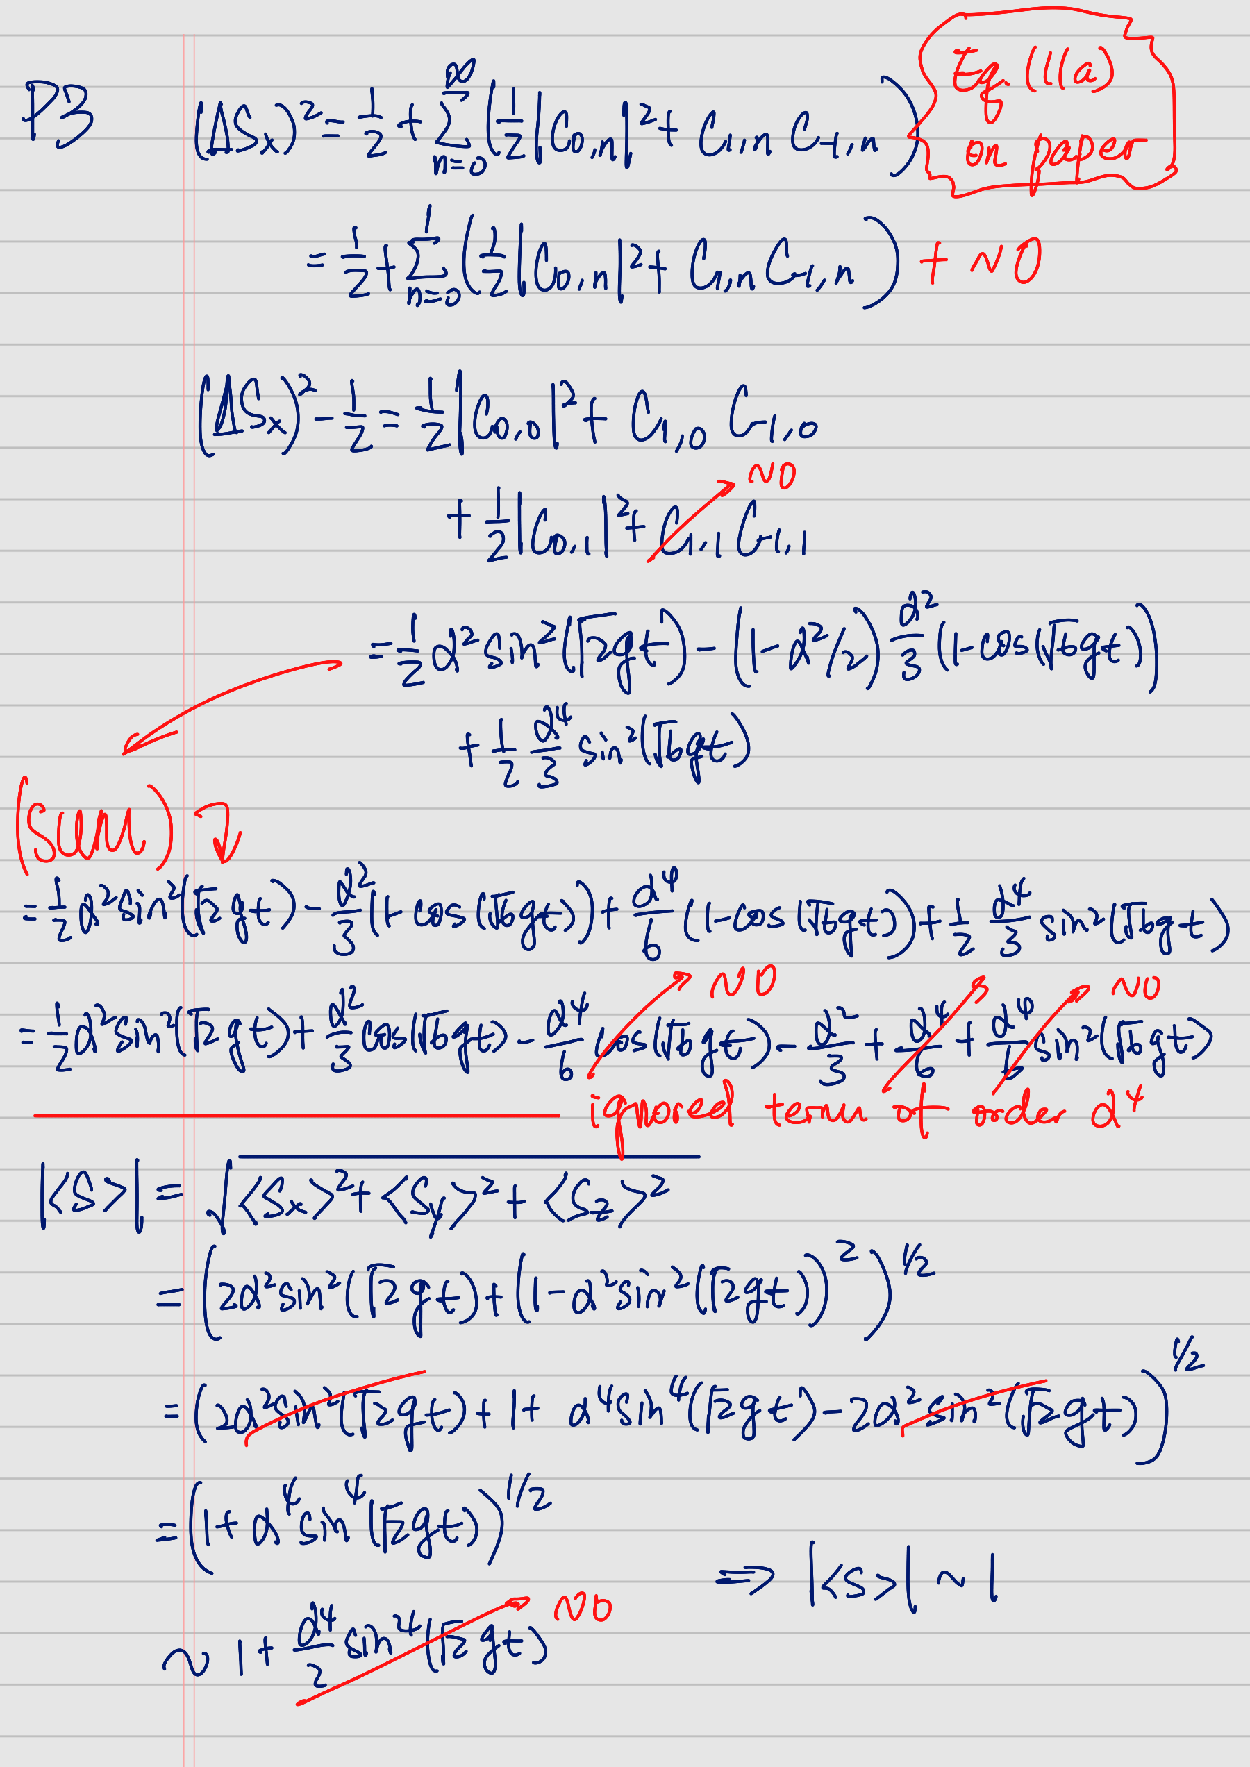
\includegraphics[scale=0.69, page=1]{542HW7_sketch}
\includegraphics[scale=0.69, page=2]{542HW7_sketch}
\end{center}


\end{document}



